\section{Conclusion and future work}
\subsection{Conclusion}
Developing a bridge builder was harder than we thought. During the process of making the bridge builder we encountered unexpected problems for which we had to find solutions. We were not able to implement all solutions, but in the future work we will describe how we would have implemented those solutions if we had more time. \\

The biggest problem was to make it easy to use, but at the same time giving a lot of freedom. The user is now unable to build in each direction he wants, but that makes it easier for him to connect the building blocks. If we did let him build in each direction, then it is easier to make small mistakes that can be troublesome at the other side of the bridge. When we started the project we thought our biggest problems would be the technical aspects of the game, but during the project we realized how hard it is to find the right balance between two different aspects of the game.  \\

We only had to make pretty small decisions, but we can imagine that the decisions at bigger project are much harder to make. Do they want better graphics, better performance or a combination that would increase the developing time? Do they want one long loading time or multiple smaller loading times? So compared to that trade-offs our decisions were relatively easy, so we can imagine that much more analysis has to done to make such important decisions at bigger projects.\\
\subsection{Future work}
\textbf{Different types of building blocks}\\
The most important thing that we would improve in a next version, is adding different kind of building blocks. This would greatly improve the different kinds of bridges that can be built with the bridge builder. When the user can build many different kinds of bridges, we can make the game more challenging for the user, because when there are only limited types of bridges that the user can build it is easier for the user to find the best type of bridge to build. \\
The problem we encountered with adding different kind of building blocks is that it is difficult to make them significantly different than the other building blocks. We had some ideas on how to make new building blocks different from others:\\
\begin{itemize}
\item A block that breaks in his own middle instead of at the connection points.
\item Give stronger blocks a lower score than weaker blocks.
\item Some building blocks will stretch out before they break
\item Some building blocks will break in the middle, while others should break at the connection points.
\end{itemize} 
\textbf{Limited building blocks per level}\\
Another feature that can be added is making some of the building blocks only available by a limited amount. This would limit the possible bridges that could be build, but at the same time make the game more challenging and lets users think better on how to use the building blocks instead of building a bridge with a large amount of blocks.  
It is not really hard to do it technically, but you have to look at each level to define what the limit of the blocks should be. If the limit of a level is too low it will discourage users to solve the level, but when the limit is too high there is no real challenge in solving the level.\\ \\
\textbf{Build in all directions}\\
It is only possible to build to the right, left, forward, backwards up or down. There could be made a lot of more different kind of bridges. An idea to build in every direction is to first show a horizontal circle where the users can decide in which direction he wants to build. Then another circle shows up so that the users choose if he wants to build up or down or just straight. 
\begin{figure}[H]
    \centering
    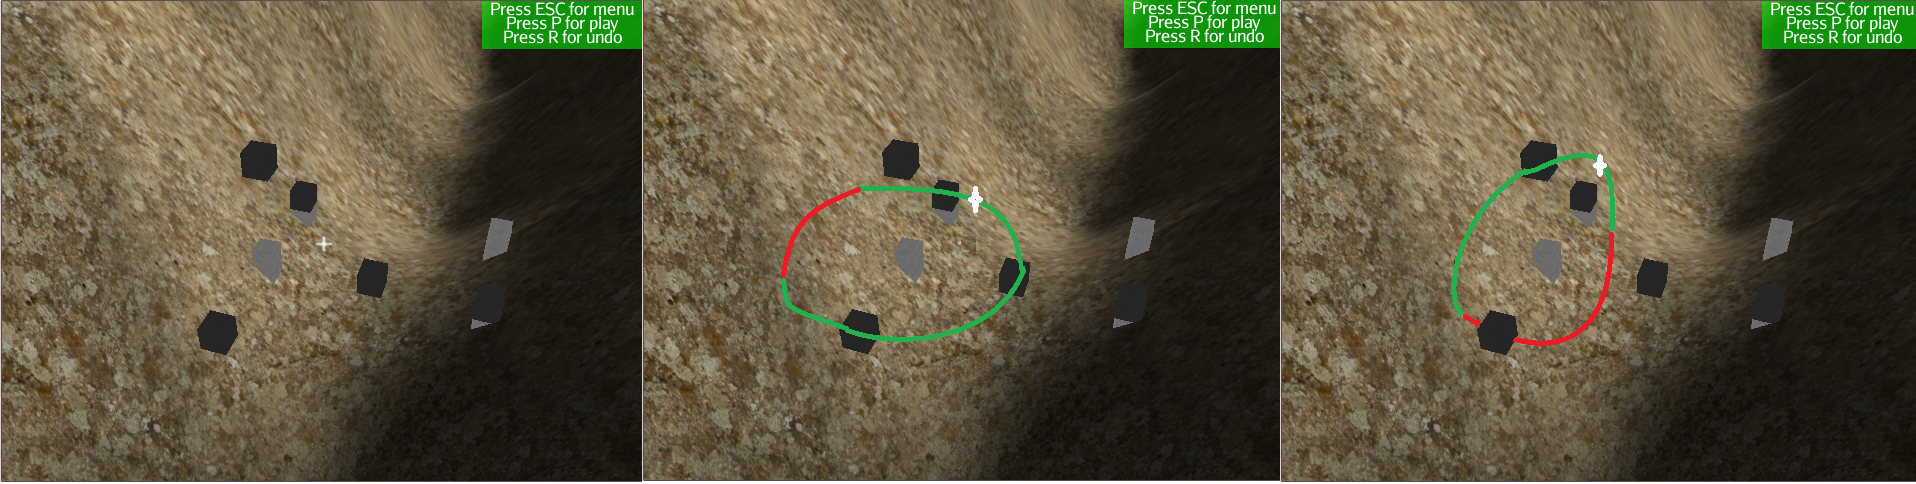
\includegraphics[width=0.8\textwidth]{screenshots/TwoClick.png}
    \caption{First screen is how it is now, second en third screen show the two clicks that have to be made to build in all directions}
    \label{fig:twoclick}
\end{figure}
This would cause some other problems. You have to check for collision, so that user does not build two building blocks that go through each other. You also have to make sure that the connection is still going good. If you are missing the other building block by a few pixels it should automatically connect to that building block, but maybe this is not always what you want.  \\ \\
\textbf{Save and load bridge}\\
A problem we encountered during testing the game is that when you build a bridge and you let the train drive over it and it collapses. You have to build the bridge again and cannot go back to the bridge before the collapsing. This really discourages the user when he spends a lot of time on a bridge that was almost perfect, but still collapsed then you have to build that bridge again to add some missing parts to make the bridge perfect. \\
The same problem occurs when you are working on a larger level and you have to go, and then you cannot continue working on that bridge when you get back. Unless you leave the program open.  This can be solved by an option to save and load your bridge. So you can save you bridge before you let a train drive over it and afterwards load that bridge so you can make it perfect.\\ \\
\textbf{More realistic world}\\
A more realistic world would make bridge builder more attractive to play. The world can be made more realistic by several improvements. 
There are not many environment details, like nature elements, buildings and humans. If these were added to Bridge Builder it would look even better.
The train could be made more realistic. This can be done by adding more details by the train, but it could also be done by loading a train model. There can be found multiple good looking train models on the internet that could be implemented in the project to get a better looking train.
The physics could be more realistic, by looking for a better balance between the mass of the train, the mass of the building blocks and the point at which building blocks fall apart. 
